\documentclass[a4paper,11pt]{custom}
\usepackage[utf8]{inputenc}
%
%--------------------   start of the 'preamble'
%
\usepackage{graphicx,amssymb,amstext,amsmath}
%
%%    homebrew commands -- to save typing
\newcommand\etc{\textsl{etc}}
\newcommand\eg{\textsl{eg.}\ }
\newcommand\etal{\textsl{et al.}}
\newcommand\Quote[1]{\lq\textsl{#1}\rq}
\newcommand\fr[2]{{\textstyle\frac{#1}{#2}}}
\newcommand\miktex{\textsl{MikTeX}}
\newcommand\comp{\textsl{The Companion}}
\newcommand\nss{\textsl{Not so Short}}
%
%---------------------   end of the 'preamble'
%
\begin{document}
%-----------------------------------------------------------
\title{
  Streaming Vidéo
}
\author{
  Robin Moussu
  \thanks{
    suppervisé par Steven Dupont
  }
}
\maketitle
%-----------------------------------------------------------
\begin{abstract}\centering
A couple of sentences on three or four lines to summarise your work.\\ 
This is a \LaTeX\ template for undergraduate project reports.\\
Its detailed contents evolve to reflect FAQs.
\end{abstract}
%-----------------------------------------------------------
\chapterimage{head1.png} % Table of contents heading image
\tableofcontents
%-----------------------------------------------------------
\chapter{Introduction}
The first chapter of a well-structured report is always an
introduction, setting the scene with motivation and context (as in
Sec.~\ref{intro}) and then looking ahead to summarise what's in the
rest of the report (as in Sec.~\ref{intro:contents}). It's the
bit that readers look at first --- {\em so make sure it hooks them!}
%
\section{Context and motivation}\label{intro}
This is a template for \LaTeX\ project reports in the Department of
Mathematical Sciences. It shows a good overall structure for the
printed document, and shows how to construct it with a master file
(\texttt{report.tex}) plus subsidiary files (\texttt{chap1.tex},
\dots, \texttt{app1.tex}, \dots, \texttt{biblio.tex}).
\par
At the same time, features of the current version of \LaTeX\ (\LaTeXe)
are illustrated --- such as mathematical expressions, numbering and
cross-referencing, bibliography and citations, graphics and tables.
Comparison of the source files with the printer-ready document will
answer a few FAQs: \Quote{How can I do \dots\ in \LaTeX?}.
\par
However, this is {\em not} a textbook on \LaTeX\ --- for that, use the
\lq\nss\rq\ notes by Oetiker \etal\ \cite{NSS}. They are written for
novices, and are a pleasure to read. They are available free on-line,
and are kept up-to-date. The \LaTeX\ book at \textsl{Wikipedia}
\cite{WL} includes the \nss\ material and is good for reference too.
Access these via the \LaTeX\ resources page \cite{LAT}.
\par
For more advanced features see \eg\lq\comp\rq\ \cite{MG}.
\par
Well-meant advice on \LaTeX\ for report-writing and poster-making is
available\footnote{From  \texttt{bob.johnson@dur.ac.uk}} in room CM315,
where there are reference copies of both \comp\ \cite{MG} and
\textsl{The Graphics Companion} \cite{GRM}.
\par
Even if you are misguided enough \cite{AC} to prepare your report in
\textsl{Word}, this template at least exemplifies a good structure ---
and gives advice about references and help with typography.
%
\section{Contents}\label{intro:contents}
The main body of this report is divided as follows.
\par
Chap.~\ref{sec:formulas} has some examples of mathematics, then
Chap.~\ref{sec:graphics} deals with graphics and includes
Sec.~\ref{sec:tables} about tables. The Conclusion, in
Chap.~\ref{andfinally}, summarises what's been achieved, the open
questions and what could be done next.
\par
Then comes the Bibliography, listing all sources of material, data and
computer programs used, \etc. Its construction is explained in
\cite[Sec.~4.2]{NSS} and there's more about it in App.~\ref{app:refs}.
\par
Otherwise appendices typically hold basic background theory, or
additional or similar examples, or longer proofs (App.~\ref{app:proofs})
 --- anything you need but which would hold up the main flow of the
story. You could also use an appendix for listings of any computer
programs that you've written (App.~\ref{app:programs}).
\par
Here there's information about using a PC (App.~\ref{app:pc}) plus
brief advice on grammar and typography (App.~\ref{app:typo}).
%

\chapter{Formulas and theorems}\label{sec:formulas}
Each main chapter or section should start with a short description of
what it holds, and why. Top tip --- begin the whole writing enterprise
with a first draft of this little bit for each chapter. It will force
you to think about overall structure.
\par
Here we get going with mathematics and show firstly some simple
equations and then some that are slightly less simple. Then there's a
theorem whose proof is relegated to an appendix, followed by some
numbered results.
%
\section{Plain}
Here's an inline formula: \(E=mc^2\), and here's the same
thing displayed:\[E=mc^2.\]A matrix needs to be displayed:
\[  \det\left(\begin{array}{cc}
        a & b \\  c & d \\
      \end{array}\right) = ad-bc,   \]
and here's a result that's displayed and labelled:
\begin{equation}\label{eq:display}
\lim_{a\to\infty}\int_0^a\exp(-x^2)\,dx=\fr12\sqrt\pi.
\end{equation}Note the punctuation in eq.~(\ref{eq:display}) \etc,
which recognises that displayed equations are parts of sentences.
\par
Note also that a smaller (\verb+\textstyle+) size of numerical fraction
is often useful in a displayed equation. The appropriate
\verb+\newcommand+ called \verb+\fr+ is defined in the
\Quote{preamble}, in file \texttt{report.tex}.
\par
More complicated limits on \verb+\int+ (and \verb+\sum+) need to
be enclosed in braces $\{\cdots\}$.
\par
In an inline formula, avoid ugly fractions such as \(v=\frac st\) and
\(\frac{dy}{dx}=x+y\). It looks much better to write \(v=s/t\) and
\(dy/dx=x+y\). That is, keep \verb+\frac+ for
display:\[\frac{dy}{dx}=x+y\]where it belongs.
\par
Beware of inadvertent blank lines in your \texttt{.tex} file; they often
creep in immediately after a displayed equation. A blank line gives a
new paragraph, usually indented, which may not be what you want. You can 
avoid blank lines altogether by breaking paragraphs with \verb+\par+
instead, as done here.
%
\section{Fancy}
Now an equation on several lines using \verb+align+:
\begin{align*}
  |\vec A|^2 &= a_1^2+a_2^2  \\
             &= \sin^2\theta+\cos^2\theta \\
             &= 1
\end{align*}--- where the star on \verb+align*+ suppresses
all line-numbering\footnote{And re-phrase material where any displayed
equation splits between pages.}.
\par
Again, with just one line numbered for reference:
\begin{equation}
\begin{aligned}
  |\vec A|^2 &= a_1^2+a_2^2  \label{line-one}\\
             &= \sin^2\theta+\cos^2\theta \\
             &= 1 
\end{aligned}
\end{equation}
Now you can refer to equation~(\ref{line-one}).
\par
If you want to number the equations in Chapter 2 as (2.1), (2.2), etc,
then\footnote{Top tip: easily find out about any \LaTeX\ command by
putting it \textit{with} its backslash (and perhaps the word \lq latex')
into your favourite search engine.} put \lq\verb+\numberwithin+' into
\textsl{Google} or see \cite[Sec 8.2.14]{MG}.
\par
Notice that in equations you use \verb+\lim+, \verb+\exp+, \verb+\sin+
and \verb+\cos+ and not plain $lim$, $exp$, $sin$ and $cos$. See
\cite[Sec.~3.3]{NSS} for a list.
\par
For a lot of complicated multi-line formulas it's better to use the more
sophisticated display environments provided by the package
\texttt{amsmath} --- see Sec.~8.2 of \comp\ \cite{MG}.
For instance the \texttt{cases} environment is used to get
\[\theta(x)=\begin{cases}0&\text{if $x<0$,}\\
		1&\text{if $x>0$.}\end{cases}\]
And if you need continued fractions, instead of 
\[x=\frac{1}{a_2+\frac{1}{a_3+\frac{1}{a_4+\cdots}}},\]a better-looking
result
is\[x=\frac{\strut1}{\displaystyle a_2+\frac{\strut1}{\displaystyle
a_3+\frac{\strut1}{\displaystyle a_4+\cdots}}},\]for which
\texttt{amsmath}
provides the command \verb+\cfrac+ \cite[Sec.~8.4.2]{MG}.
\par
The package \texttt{amssymb} \cite[Chap.~8]{MG} extends the range of
mathematical symbols (\eg\(\mathbb{R}\), \(\mathbb{Z}\) and
\(\mathbb{N}\) are available).
\par
And its sister \texttt{amstext} provides the command \verb+\text+ to
put words into a displayed equation \[ \text{like this: }E=mc^2. \]Note
that you need to put in by hand the spacing between the text and the
mathematical symbols.
%
\section{Theorems}\label{angels}
This is theorem~\ref{angels}.
\begin{description}
\item[Theorem]: The whole is greater than the sum of its parts.
\item[Proof:] See App.~\ref{app:proofs}, Sec.~\ref{pf:angels}.
\end{description}
For numbered theorems, use \verb+\newtheorem+ \cite[Sec.~3.8]{NSS}.
\par
Here's the main sequence of theorems.
\newtheorem{Main}{Theorem} % this could go into the preamble
\begin{Main}[my first result]
The first theorem, showing
\[ \bar D^n\quad\text{and}\quad\bar{D^n} \]
where the first bar is over just the \lq D\rq\ and the second is over
the whole expression. Also the word \lq and\rq\ is inside displayed
maths, using \verb+\text+ with extra space before and after.
\end{Main}And that's how to do left and right quotation marks, too,
with \verb+\lq+ and \verb+\rq+.
\begin{Main}
The second theorem --- with \verb+\overline+ inline: $\overline{D^n}$.
\end{Main}
\begin{Main} the third theorem\end{Main}
Here's another sequence of results.
\newtheorem{second}{Lemma} % this too could go into the preamble
\begin{second}[my second result]
The next result (a mere lemma) \dots\end{second}
\begin{second}\dots\ and the next\end{second}
\comp\ \cite[Sec.~3.3.3]{MG} describes how to use the
packages \texttt{amsmath} and \texttt{amsthm} to state (and
cross-reference) theorems, lemmas, definitions, proofs, \etc\ in a more 
sophisticated way.
%
\section{Summary}
Each chapter should end with a round-up of its contents and a link
with the contents of the next.
\par
After formulas, equations and theorems, the next important
topics are graphics and tables.

\chapter{Graphics and tables}\label{sec:graphics}
\chapterimage{head1.png} % Table of contents heading image
Graphics files are inserted via the package \texttt{graphicx} which is
loaded in the document preamble (in file \texttt{report.tex}).
\par
Here we deal firstly with the inclusion of a single unlabelled diagram,
and then with captioned, labelled, and multiple diagrams.
\par
After that we consider tables of information.
%
\section{Plain}
Here is a colour \texttt{.jpg} file, inserted in place without caption
and without a number for cross-reference. It's suitable only for a
simple self-explanatory diagram, used here and not again.
\begin{center}
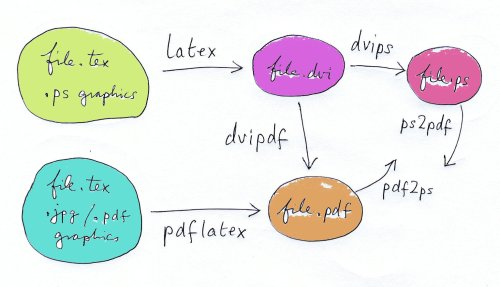
\includegraphics[width=.7\textwidth]{pic1.jpg}
%\includegraphics[width=.7\textwidth]{pic1new.jpg}
\end{center}
It shows the normal routes from a \LaTeX\ source (\texttt{.tex} file) to
\texttt{.ps} or \texttt{.pdf} output depending on the nature of the
graphics files included\footnote{An IDE such as TeXnicCenter has menu
buttons for each part of each route.}. \textit{Confusion over these
routes is a frequent source of grief}.
\par
This template has diagrams and graphs in \texttt{.jpg}
format\footnote{File extensions must be \texttt{.jpg} and not
\texttt{.JPG} or \texttt{.jpeg}.} and so its source is compiled to a
\texttt{.pdf} file with the command or menu button \texttt{pdflatex}.
\par
Mathematical software such as \textsl{Maple} and \textsl{Matlab} can
produce either \texttt{.ps} or \texttt{.jpg} diagrams, while cameras and
scanners\footnote{The figure itself is hand-drawn and scanned.} usually
produce \texttt{.jpg}. If accurate detail is vital, \texttt{.ps} is
best.
\par
With care, you can mix some graphics formats within a document. For
instance, if you compile to \texttt{.pdf} then you can use an
arbitrary mix of \texttt{.jpg}, \texttt{.png} and \texttt{.pdf}
graphics, but not \texttt{.ps}. And a document to be compiled to
\texttt{.dvi}, including \texttt{.ps} graphics, can include other
formats too if they are explicitly given \Quote{bounding boxes}. But
it's relatively tricky and you're better-off converting everything to
one format.
\par
Note that you can't include \texttt{.bmp} or \texttt{.gif} files at
all, but conversion of graphics files --- from \texttt{.bmp} to
\texttt{.jpg} for example --- is easily done with software like
\textsl{PhotoShop} \cite{PS} or \textsl{ImageMagick} \cite{IM}.
\par
It's simplest to keep your image files in the same directory as your
\texttt{.tex} files. Otherwise you can explore the mysteries of
\verb+\graphicspath+ \cite[Sec.~10.2.5]{MG}. In any case, use only
forward slashes in a directory specification. Names of directories and
of graphics files \textit{must not} include spaces!
%
\section{Fancy}
It's awkward to flow text round a picture, but it can be done with
packages such as \texttt{picinpar} or \texttt{wrapfig}, as \comp\
explains \cite[Sec.~6.4.1]{MG}.
\begin{center}
\begin{minipage}[c]{.45\textwidth}\centering
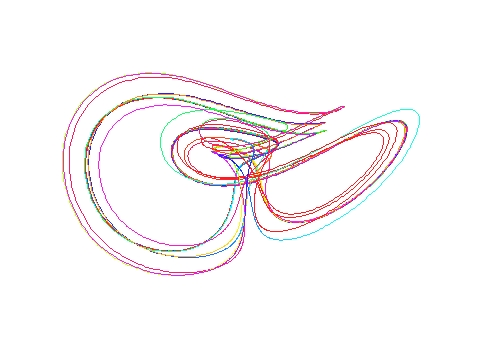
\includegraphics[width=.9\textwidth]{pic2.jpg}
\end{minipage}
\hfill\begin{minipage}[c]{.45\textwidth} And here's a \texttt{.jpg}
image side-by-side with some explanation, using the \texttt{minipage}
environment.\end{minipage}\end{center}
Something more elaborate sometimes gives unexpected results.
\par
\begin{figure}[ht]\centering
  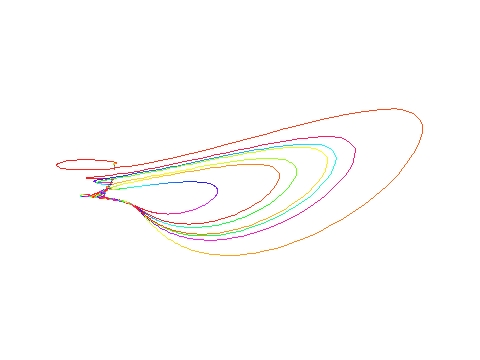
\includegraphics[width=.7\textwidth]{pic3.jpg}
  \caption{This is a caption explaining the diagram 
clearly and fully.}\label{fig:pic}
\end{figure}
That is, a picture \lq floating\rq\ in a \texttt{figure} environment
--- with a caption and number as in Fig.~\ref{fig:pic} --- might be
placed by \LaTeX\ on a page well after the text meant to accompany it.
\par
This happens if you have a relatively high density of graphics to
text. You may be able to deal with it by re-distributing the
pictures, changing the size of some of them, and the careful use of
paragraph breaks. Otherwise you may resort to \verb+\clearpage+,
which forces insertion of floating objects waiting to go in.
\par
The \nss\ book \cite{NSS} has Sec.~2.12 on the issue of \lq floating
bodies\rq\ and \comp\ has a whole chapter \cite[Chap.~6]{MG} on \lq
mastering floats'.
\par
Note that inside a \verb+figure+ (or \verb+table+) environment the 
\verb+\label+ must always {\em follow} the \verb+\caption+ --- see 
\cite[p.~67]{MG}.
\par
\begin{figure}[ht]\centering
\begin{minipage}[c]{.45\textwidth}\centering
  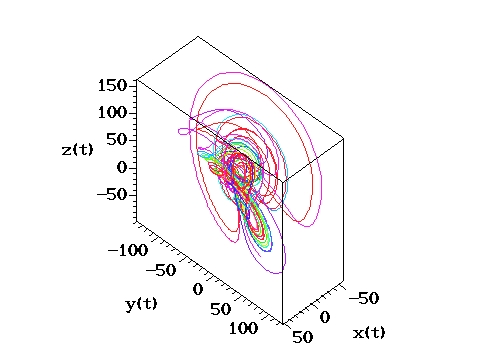
\includegraphics[width=.95\textwidth]{pic4.jpg}
  \caption{Caption to explain the diagram 
clearly and fully.}\label{fig:pictwo}
\end{minipage}\hfill
\begin{minipage}[c]{.45\textwidth}\centering
  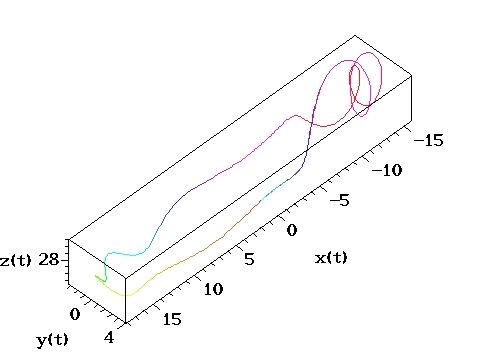
\includegraphics[width=.95\textwidth]{pic5.jpg}\\
  \caption{Caption to explain the diagram
clearly and fully.}\label{fig:picthree}
\end{minipage}
\end{figure}
Fig~\ref{fig:pictwo} and Fig.~\ref{fig:picthree} are two pictures
floating side-by-side, each in a \texttt{minipage} and each with its
own caption and label. This can be an economical way to insert multiple
diagrams.
\par
But don't get carried away and cram too many pictures together.
Be aware of the size-reduction that's often necessary, and maintain
legibility by choosing large enough font and weight for symbols,
axis-labels and other text.
\par
Figure captions should give plenty of information, because readers will
first skim the Introduction and Conclusions --- and then look at the
pictures. If you want (really really want) to hook them, make sure that
every important figure plus its caption is as self-explanatory as
possible.
%
\section{Tables}\label{sec:tables}
Besides figures you may want to include tables. Like figures, tables may
be plain and simple --- short and for immediate and local use only ---
and so put in place without a caption or label; or they may be
complicated and important enough to need a reference label and an
explanatory caption. Here are examples of each in turn.
\par
First a simple table \dots\par
\begin{center}
 \begin{tabular}{|l||c|c|c|r|}
    \hline
    row 1& it's & just & as & easy \\ \hline
    row 2& as & this & \(E=mc^2\) & what \\ \hline
    row 3& could & be & simpler & ? \\ \hline
    row 4& as & easy & as & \(\Pi\) \\ \hline
  \end{tabular}
\end{center}
\par
Here it is again, now floating in a \texttt{table} environment, with
a caption and a label to identify it as Table~\ref{table:one}.
\begin{table}[h]
  \centering
\begin{tabular}{|l||c|c|c|r|}
    \hline
    row 1& it's & just & as & easy \\ \hline
    row 2& as & this & \(E=mc^2\) & what \\ \hline
    row 3& could & be & simpler & ? \\ \hline
    row 4& as & easy & as & \(\Pi\) \\ \hline
  \end{tabular}
  \caption{Floating table, with a caption to explain it 
clearly and fully.}\label{table:one}
\end{table}
The remarks about giving full information in figures and their
captions apply equally to tables, of course. So do the remarks about
unexpected placement of floating objects.
\par
If you need a long table, occupying more than a page, and which
can't reasonably be divided, then you need to delve into \comp\
\cite[Chap~5]{MG} to find the secret.
%---------
\section{Summary}
Graphics files are evidently straightforward to include. If you need
to go beyond the basics, then refer to \Quote{The Graphics Companion}
\cite{GRM}.
\par
Tables are easy to use too, but don't misuse them. Lengthy data-sets can
be supplied separately on CDrom. Put only summaries in the report,
perhaps as an Appendix.

\chapter{Conclusion}\label{andfinally}
The last chapter of a well-structured report reviews what's been done and
mentions the main open questions.  It's the part a typical reader looks
at second, after the Introduction, and it should be just as appealing.
\par
This template is provided only to help you start with \LaTeX\ and to
exemplify good structure. When you've got some practice, you'll want to
alter it to suit your topic and your taste --- and you are free to do
that.
\begin{itemize}
    \item\verb+\documentclass[a4paper,twocolumn,10pt]{article}+
    gives an attractive alternative framework, for example.\par Or you
may prefer \verb+\documentclass{memoir}+ which has an excellent
manual \cite{MEM} that includes a general introduction to typography.
    \item Try to resist the temptation to make margins narrower
    and lines longer --- it may save a sheet or two of paper but it
    can make the text hard to read. Indeed, typesetting professionals 
    quote a maximum of 66 characters per line as an ideal for easy reading
          \cite[Sec.~5.2.2]{NSS}.
    \item proof-read carefully --- not only to get the best from \LaTeX\
but also to polish grammar, spelling and punctuation \cite{ESL}.
App.~\ref{app:typo} alerts you to common pitfalls.
\end{itemize}
Good layout and use of \LaTeX, plus fluent and grammatical writing, will
together give a very good impression.
\par
Top tip --- write what you think is the final version, then put it
away in a drawer and come back to it a week or so later. With fresh
eyes you'll see many potential improvements. This works for anything you
prepare, not just a project report. It needs forward planning of
course!
\section*{Acknowledgements}
\addcontentsline{toc}{chapter}{\numberline{}Acknowledgements}
Here's the place for thanks to anyone who particularly helped you.
Don't go too far OTT --- try to keep some dignity. This isn't the 
Oscars.


%-----------------------------------------------------------
\addcontentsline{toc}{chapter}{\numberline{}Bibliography}
\begin{thebibliography}{9999}%\enlargethispage{\baselineskip}
\bibitem[AC]{AC}A~Cottrell, \textsl{Word Processors: Stupid and
Inefficient},
\\ \mbox{}\hfill\texttt{www.ecn.wfu.edu/\~{}cottrell/wp.html}
\bibitem[BR]{BR}Visit \texttt{www.dur.ac.uk/library/using/guides/}
and click on \Quote{Writing your bibliography and citing references}.
\bibitem[ESL]{ESL}L~Truss, \textsl{Eats, Shoots and Leaves}, Profile
  Books 2003\\ \mbox{}\hfill(ISBN~\texttt{1-86197-612-7}).
\bibitem[GRM]{GRM}M~Goossens, S~Rahtz and F~Mittelbach,\\
  \mbox{}\hfill \textsl{The \LaTeX\ Graphics Companion},
  Addison-Wesley, 1997\\  \mbox{}\hfill(ISBN~\texttt{0-201-85469-4}).
\bibitem[IM]{IM} \textsl{ImageMagick}, {\tt%
www.dur.ac.uk/its/software/application/\dots
\\ \mbox{}\hfill\dots?application=ImageMagick}
\bibitem[LAT]{LAT} \textsl{\LaTeX\ stuff},
	\texttt{maths.dur.ac.uk/Ug/projects/resources/latex/}
\bibitem[MEM]{MEM} \textsl{Memoir document class},\\ \mbox{}\hfill
   \texttt{www.ctan.org/tex-archive/macros/latex/contrib/memoir/}
\bibitem[MG]{MG}F~Mittelbach and M~Goossens \etal, \textsl{The
\LaTeX\ Companion},\\  \mbox{}\hfill Addison-Wesley, 2nd ed. 2004
(ISBN~\texttt{0-201-36229-6}).
\bibitem[MKT]{MKT} \textsl{MikTex Project Page}, \texttt{www.miktex.org}
\bibitem[NSS]{NSS}T~Oetiker, H~Partl, I~Hyna and E~Schlegl,\\
\mbox{}\hfill
\textsl{The Not So Short Introduction to \LaTeXe},\\ \mbox{}\hfill{\tt
www.ctan.org/tex-archive/info/short}
\bibitem[PS]{PS} \textsl{Photoshop}, {\tt%
www.dur.ac.uk/its/software/application/\dots
\\ \mbox{}\hfill\dots?application=Adobe+Photoshop}
\bibitem[TXC]{TXC} \textsl{TeXnicCenter}, \texttt{www.toolscenter.org}
\bibitem[WDT]{WDT} \textsl{WinEdt}, \texttt{www.winedt.com}
\bibitem[WL]{WL} \textsl{Wikibook on \LaTeX}, \texttt{%
	en.wikibooks.org/wiki/Latex}
\bibitem[WO]{WO} \textsl{Controlling widows and orphans}, 
\\ \mbox{}\hfill\texttt{www.tex.ac.uk/cgi-bin/texfaq2html?label=widows}
\bibitem[WSH]{WSH} \textsl{WinShell}, \texttt{www.winshell.de}
\end{thebibliography}
\vfill
\begin{flushright}\small Prepared in \LaTeXe\ by RCJ\end{flushright}

%-----------------------------------------------------------
\appendix
\chapter{About references}\label{app:refs}
Your report will be put together in your own style, mostly using your
own words. Much of it will be standard material that you've read and
digested, but you may have a fresh example, application or calculation
that you've done yourself.
\par
You must make clear what's not your own work by referring suitably
to your sources --- books or articles or web-pages, etc. Not to do so
can count as plagiarism, which is cheating.
\par
This appendix aims to amplify the advice given in the
Library's guide \cite{BR}, which you should read.
%----------------------------------------
\section{Organisation}
Follow the style of this template --- that is, put an orderly list of
your sources (\Quote{The Bibliography}) at the end of the main text,
and refer to (\Quote{cite}) items on the list by suitable codes placed
appropriately in the report's text.
\par
For your bibliography the golden rule is that each listed item must give
enough detail to allow readers to follow it up themselves and find the
precise part of the book, article, web-site or whatever without
ambiguity or delay.
\par
For instance it's no use saying just \Quote{The Times newspaper} unless
you also give the date and page, or just \Quote{Wikipedia} unless you
give the complete URL of the specific page, \dots\ and so on.
\par
It's always better to give slightly too much information --- e.g. you
might include the ISBN of a book too. A good level of information is
exemplified here and recommended in the Library guide \cite{BR}.
\par
If you need to cite different parts of e.g. a book for different things,
then list it (say AB) in the bibliography and give the different
citations as [AB,~page~32] and [AB,~Sec.~4.7] and so on. The \LaTeX\
\verb+\cite+ command allows for this (look it up!).
\par
Now you see why a bibliography list is better than lots of footnotes
--- it neatly allows such multiple citations. Too many footnotes make a
mess.
\begin{itemize}\item This bibliography uses short letter-code
keys in alphabetical order. It's one of several standard possibilities
\cite{BR} and is often preferred for economy and because the letter
codes\footnote{Note the punctuation of \lq letter-code' and \lq letter
codes' here.} can be chosen to be helpful mnemonics. Numerical codes,
for instance, can't.
\item Long lines (with URLs usually \cite{IM,PS}) may need to be split.
The \LaTeX\ hack used here to manage such line-breaks may not appeal to
everyone.\end{itemize}
%---------------------------------
\section{Doing it}
What things need a reference? The answer is --- anything you didn't work
out or invent yourself, but took from someone or somewhere else. You may
do that, so long as you say so \textit{and also make it clear you
understand it}. Don't copy blindly! Here are some
examples.\begin{itemize}
\item \Quote{the following explanation is taken from [LH]} --- if you've
copied word-for-word from the article by Laurel \& Hardy, which you
list as item LH in the bibliography. Direct quotation should be used
sparingly, and the text emphasised --- perhaps by use of the
\texttt{quotation} environment in \LaTeX.\par
Don't be tempted to copy from a book, or \texttt{ctrl-C/ctrl-V} from the
web, \textit{without} clearly admitting it. It's easy to detect, and
it's suicide.
\item \Quote{the following proof is in many textbooks, \eg
[LH,~page~16]} --- if it is, and you can't think of a different proof,
except perhaps for notation.
\item \Quote{the material in this section is based on Sec.~2.6 of [CL]
and Chap.~3 of [SH]} --- if you've combined into your own words the
account by Cagney \& Lacey with that by Starsky \& Hutch.
 \item \Quote{the following proof is adapted from Chap.~4 of [SJ]} ---
if (say) you've filled in the gaps in Smith \& Jones' proof, or perhaps
changed it from the case of general $n$ to your case $n=2$.
\item \Quote{these calculations were done with \textsl{Matlab} [MAT]
using the m-file listed in App.~\ref{app:programs}} --- where the
reference MAT is to the \textsl{MathWorks} website.
\item \Quote{these calculations were done with the TISEAN package [TIS]}
--- if you've downloaded this specialised package from a web-page whose
URL (and author's name, if available) is item TIS in the bibliography.
\item \Quote{the graph is taken from Morecambe \& Wise [MW, page 16]}
--- if you've scanned the figure from their book. Similarly, if you've
downloaded a \texttt{.jpg} file from a web-site, then give in the
bibliography the URL and author (if known). Such citations could go
either in the figure caption or in the associated text.
\item \Quote{the data are taken from [XY]} --- where XY gives the
source of the numbers you've analysed. This might be a journal or
an online databank, \etc. Generally the numbers themselves should be
left out
--- a summary table or a graph or two (plotted with \textsl{R} or
\textsl{Matlab} or \textsl{Maple}) is often enough. Occasionally raw
data might be supplied separately --- e.g. on a CDrom.
\end{itemize}
Often your supervisor or someone else gives you something --- such
as a set of data, or a useful \textsl{Maple} worksheet, or help with a
proof --- when the appropriate form of bibliography item is
\Quote{Dr~I~Newton, private communication, April 2007}. Similarly for
printed course material --- \Quote{Dr~I~Newton, lecture notes
for module MATH5033, Durham University, Epiphany Term 2007.}
\par
Generally, don't refer to things you haven't read. Textbooks may well
cite the Serbian-language journal where the result you want was
originally published. But you are not in the business of ascribing
credit for discovery. In \textit{your} report \textit{you} must cite the
book where \textit{you} actually got it from and not give any possibly
false impression that you fluently read technical Serbian.
\par
Likewise, you may want to quote from Euclid or Archimedes.
But cite the place where you found the English words with something like
\Quote{Archimedes said, \lq Eureka!\rq\ (as quoted by [AB])}.
\par
Summarising --- tell the truth (where you got it from), the whole truth
(give full details), and nothing but the truth (you don't read Serbian).
\par
Finally, if in doubt --- ask your supervisor.

\chapter{Long proofs}\label{app:proofs} An Appendix is a good place
to put lengthy proofs that must be included but would impede the
flow if placed in the main text.
\section{Proof of theorem \ref{angels}}\label{pf:angels}
By inspection.

\chapter{Computer programs}\label{app:programs}
An Appendix is the place to list computer programs that you've
written, using the {\tt verbatim} environment \cite[Sec.~2.11.4]{NSS}.
\par
For example ---
\begin{verbatim}
    10 PRINT "HALLO SAILOR!"
    20 GO TO 10
\end{verbatim}

\chapter{Using a PC}\label{app:pc}
You may want \LaTeX\ on your own computer.
\par
A popular version of \TeX/\LaTeX\ for a Windows PC is \Quote{MikTex}
\cite{MKT}. \miktex\ is free, and is available online for 
download \cite{LAT} or locally on a DVD from
\texttt{bob.johnson@dur.ac.uk}, room CM315. It's also installed on the
ITS Networked PC Service under \texttt{Programs | Miscellaneous}.
\par
To use \miktex\ easily you need a dedicated
editor or IDE\footnote{Computer scientists say \lq Integrated 
Development Environment'.}. A good one is \Quote{WinEdt} \cite{WDT}, 
which runs under all recent versions of Microsoft Windows and integrates 
well with \miktex. \textsl{WinEdt} is free for 31 days; to use
it thereafter costs about \$40.
\par 
Completely free rivals include \Quote{TeXnicCenter} \cite{TXC}, which is
provided on the \miktex\ DVD and also set up on the ITS Networked PC
Service under \texttt{Programs | Miscellaneous | MikTeX}.
\par
Others include \eg \Quote{WinShell} \cite{WSH}, but are untried.
\par
All these editors/IDEs have a familiar style of graphical user-interface
with a toolbar and pull-down menus for all the common tasks involved in
editing source files, running \LaTeX\ and viewing the results.

\chapter{Typography and grammar}\label{app:typo}
Some errors crop up time and again, and a few of the commonest ---
mostly relating to use of \LaTeX\ --- are mentioned in the body of this
template. Some others are given here, aiming to help you avoid them.
\par
Layout errors include starting a sentence with a symbol, or leaving a
single symbol that ends a sentence hanging alone on a line. Related to
this are \Quote{widows} and \Quote{orphans} \cite{WO}. Can you spot any
in this template?
\par
Grammar --- illiteracy makes good mathematical work look like rubbish.
Of course, everyone makes mistakes, but a final version with many small
errors in fact signals \Quote{I am ignorant and I just don't care}.
Read, mark, learn, and inwardly digest the wisdom of the great goddess
Truss \cite{ESL}.
\par
Apart from spelling blunders, the top five usual suspects in recent
project reports are (in random order) ---\begin{itemize}
\item \Quote{sentences} with no verb;
\item mis-use of apostrophes;
\item mis- or non-use of hyphens;
\item writing \Quote{comprises of};
\item unpunctuated displayed equations.
\end{itemize}
A tip for proof-reading --- a friend or relative may spot things you've
become blind to. And remember in practise their are a massive number of
errors in grammer and stile, and so fourth its only to easy to make that
you're spell checker on it's own wont find (14 in this sentence).
%----------------------------
%-----------------------------------------------------------
\end{document}
